\documentclass[a4paper]{article}

\usepackage[english]{babel}
\usepackage[utf8]{inputenc}
\usepackage{amsmath}
\usepackage{graphicx}
\usepackage[colorinlistoftodos]{todonotes}
\usepackage{graphicx}
\graphicspath{ {./images/} }

\title{Neural Network Language Models for Automatic Speech Recognition}

\author{Aditya Kaushik, Eduardo Rosado, Thomas Spilsbury}

\date{\today}

\begin{document}
\maketitle

\begin{abstract}
In this paper we compare Recurrent Neural Network (RNN)
approximations of language models to traditional n-gram based models.
We evaluate different recurrent model architectures, hyperparameter configurations,
encoder and decoder configurations and regularization and intialization procedures
while comparing their performance on various performance and natural language
generation metrics. We find that in general, Long Short-Term Memory models
with embedding layers at the encoder stage outperforms other models
in terms of inference metrics and computational performance.
\end{abstract}

\section{Introduction}
\label{sec:introduction}

One important problem faced by Automatic Speech Recognition (ASR)
systems is transcribing utterances by speakers into intelligible written language.
In general, this is a difficult problem to solve due to the varying length
of utterances and ambiguity of classification between one utterance for another. The result
is that the recognized transcript is likely
to contain many words that are not
intelligible, even if the transcribed words
are the system's most likely direct
transcription from sounds to syllables.

As an alternative, we can make use of prior
information about the language to select
words from a vocabulary given some
observations of sounds or characters and the words
that have been predicted beforehand. The language model,
then, uses information about the sequence of prior
predicted words to give a probability distribution
for the next word, such that the ASR system would
pick the next word based both on what are the most
likely following words given a sequence as well
as the utterance that is made by the speaker.

Prior to the introduction of RNNs, most language models used n-grams
in Hidden Markov Model chains, where it was assumed that the $k$th
word depended only on the prior $n$ words. One key problem
with this model is that the context window is of a fixed size, leading
to a horizon problem. The Horizon problem occur because a if there were a word
in the word sequence which is extremely predictive of the $(n + 1)$th
word away from the current word, that would would simply not be taken
into account in that model. Worse still, the fixed size context window
means that unnecessary weight is put on words that happen to be in the context
window that may actually not be all that predictive were the context window
infinite.

In contrast, RNN's seek to solve this problem by introducing a Neural Network
architecture with recurrent connections, meaning that as the RNN makes predictions
over a sequence observations, it takes into account a hidden layer produced
by the previous observation (which in turn was a product of all the observations
before that). In effect, the RNN architecture encodes the contextual history
into the hidden layer vector allowing for an encoded approximation of infinite
contextual history.

One of the first papers applying RNNs to Language Modeling was \cite{Milkolov10}. But since 2010, new RNN approaches have shown
improvement on the state-of-the-art. We examine these new architectures and
techniques for future work discussed in the Milkolov paper and analyze whether their
results indicate that improvements can be made on the baseline set by the paper.

\section{Data}
\label{sec:data}

\section{WikiText}
\label{sec:wikitext}

The first dataset we use is the WikiText dataset. This is a smaller dataset than
Gigaword and WSJ'92, but allowed us to
iterate faster and run more experiments.

This dataset is based on articles from Wikipedia, containing 1,756,924 tokens in
the training set, 184,354 tokens in the validation set and 207,080 tokens
in the test set. The combined dictionary for all three sets contains 28,755
unique tokens.

\begin{figure}[!ht]
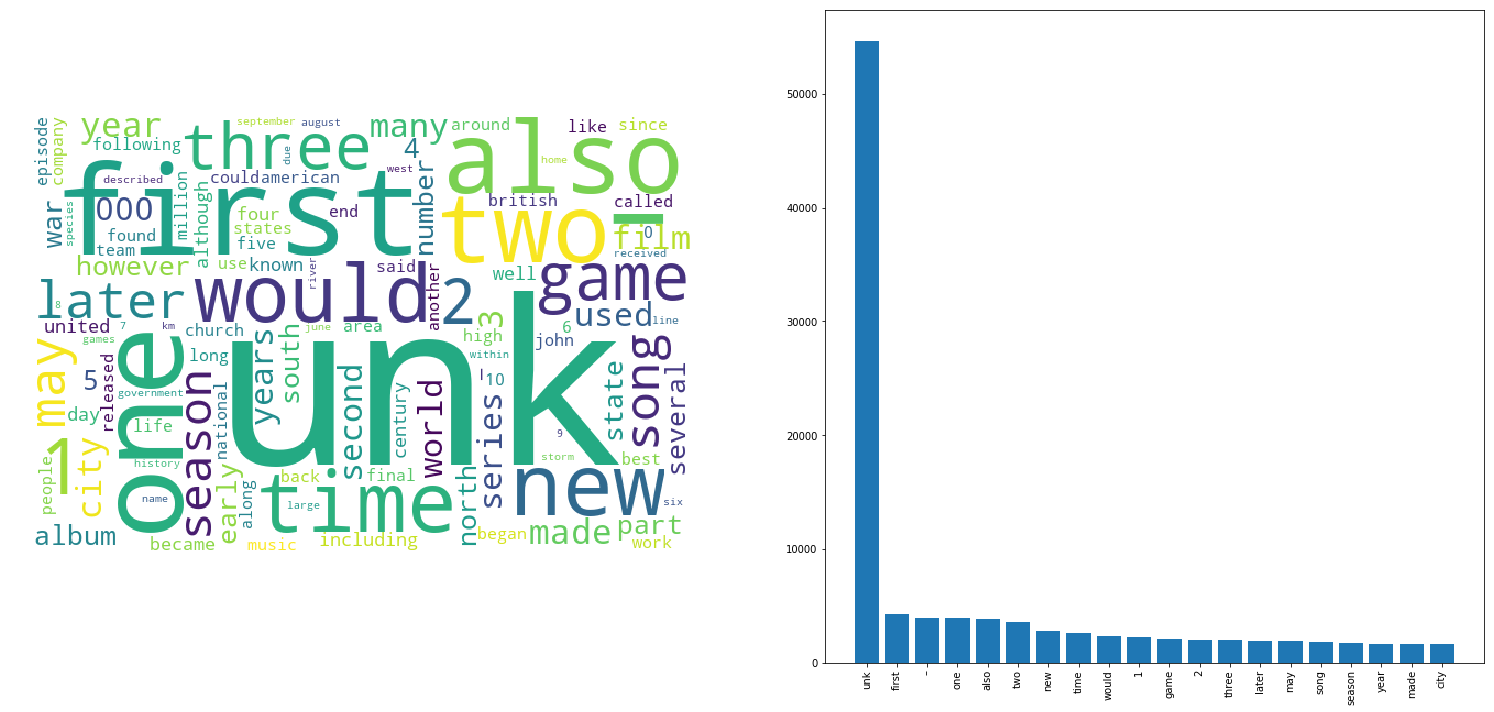
\includegraphics[width=0.7\columnwidth]{sr-eda-wikitext-train-words}
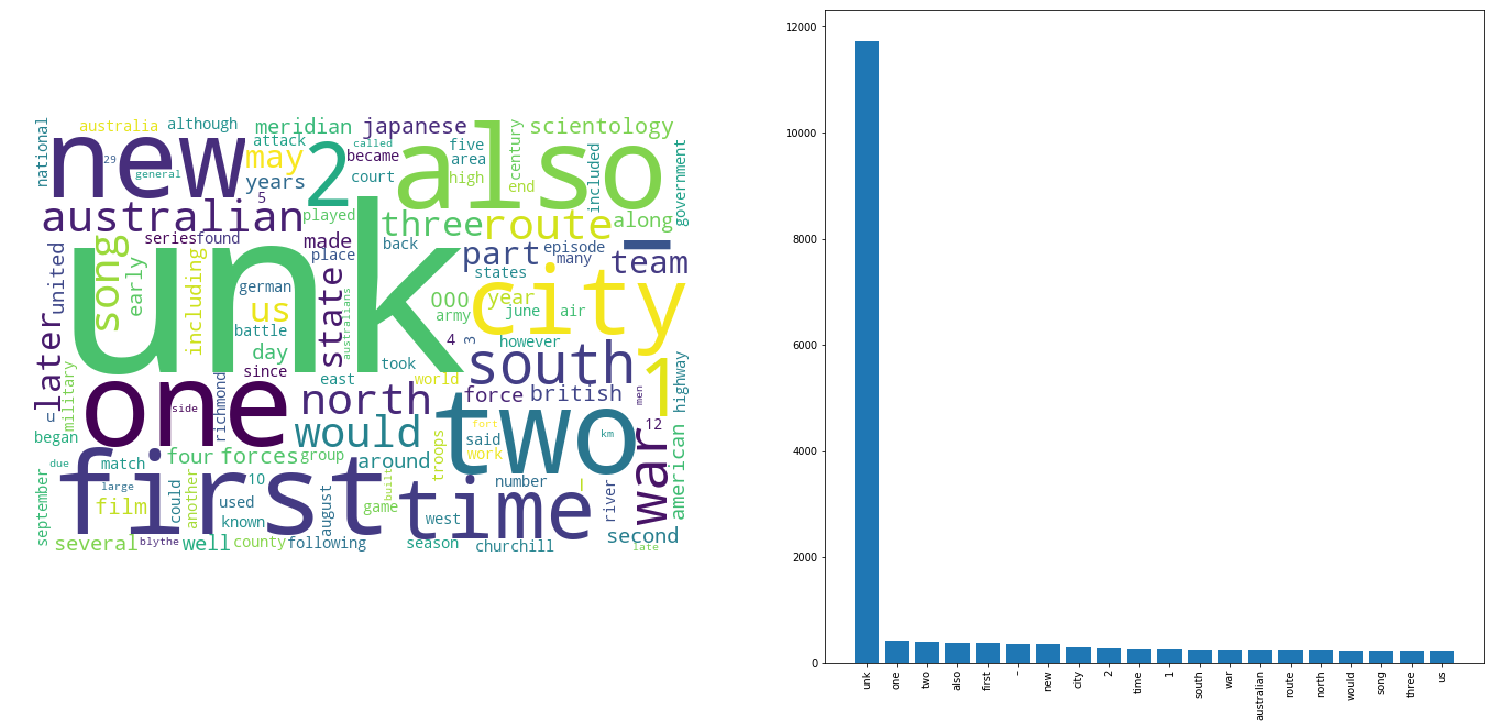
\includegraphics[width=0.7\columnwidth]{sr-eda-wikitext-valid-words}
\centering
\caption{Training and Validation words in the WikiText dataset}
\end{figure}

Notice that because of the large amount of domain specific language that is used
due to the fact that the sentences within were derived from encyclopedic
articles, the dataset contains a large number of "unknown" tokens. An "unknown"
token, represents any token with a frequency below the dataset threshold. This
inherently makes accurate prediction difficult, since there is a higher
likelihood that the following word might be infrequent in the corpus.

Samples from the Dataset include:

"As with previous <unk> Chronicles games , Valkyria Chronicles III is a …"

"At Nintendo CEO Hiroshi Yamauchi 's request , Game Boy creator Gunpei Yokoi 's Nintendo R \& D1 developed …"

"It was larger than the Scientific , at 73 by 155 by 34 millimetres ..."

Also notice the most frequent bigrams and trigrams of the dataset

\begin{figure}[!ht]
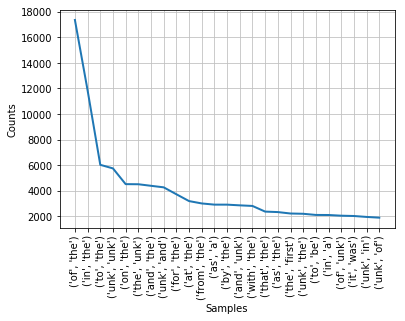
\includegraphics[width=0.7\columnwidth]{sr-eda-wikitext-bigrams}
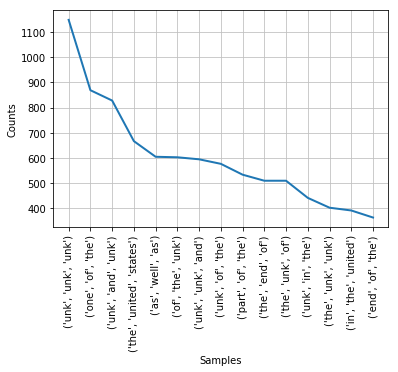
\includegraphics[width=0.7\columnwidth]{sr-eda-wikitext-trigrams}
\centering
\caption{Training set Bigrams and Trigrams in the WikiText dataset}
\end{figure}

The bigrams and trigrams in the dataset indicate that the dataset is, as expected,
most describing phenomena or objects, with large frequencies for bigrams
such as "in the" or "of the". The trigrams also reveal that domain specific
descriptions-in-general are frequently occurring, ("unk unk unk").

\section{Gigaword}
\label{sec:gigaword}

The second dataset we used was Gigaword. This dataset is based on XXX,
containing 110,382,986 tokens in the training set, 549,0454 tokens in the
validation set and XXX tokens in the test set. The combined dictionary
contains XXX unique tokens.

Samples from the Dataset include:

XXX

\begin{figure}[!ht]
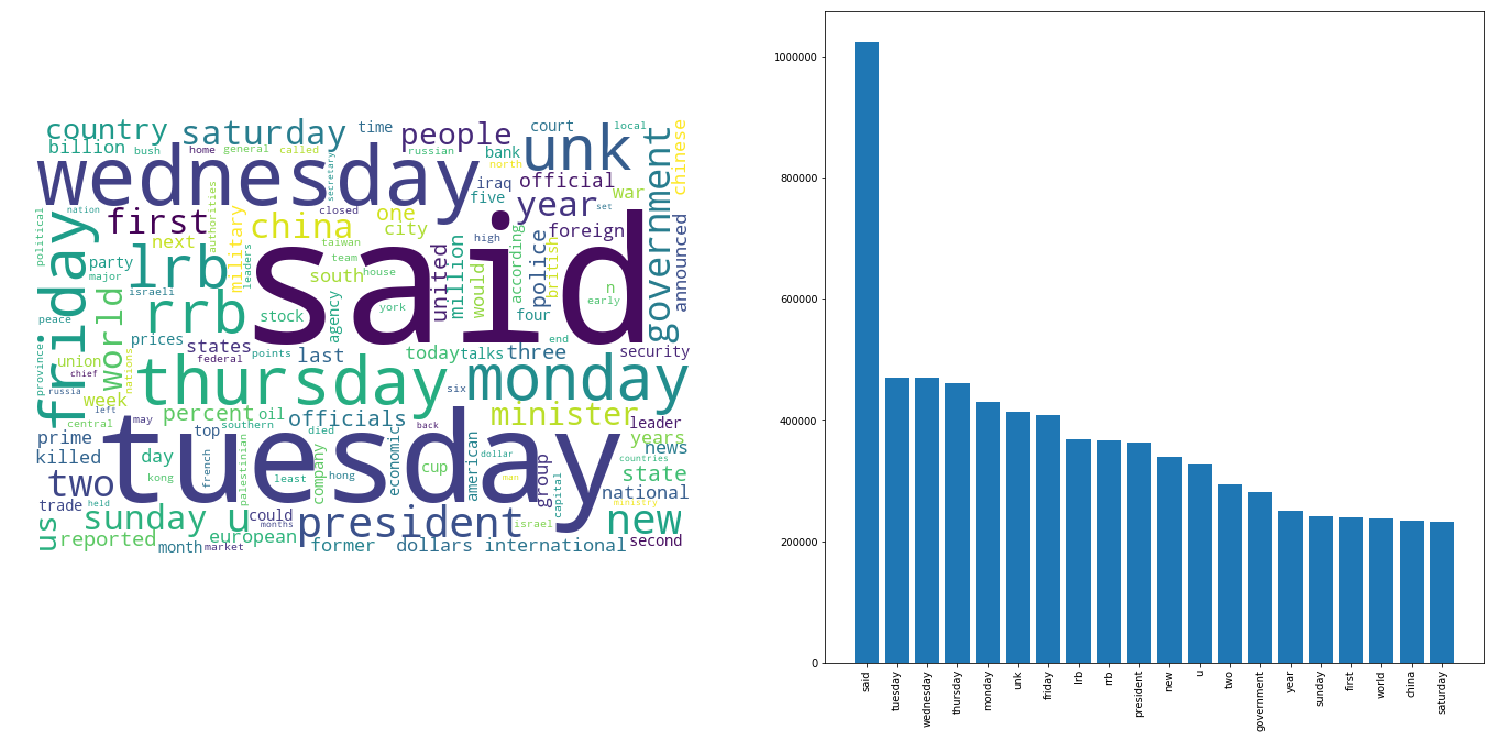
\includegraphics[width=0.7\columnwidth]{sr-eda-gigaword-train-words}
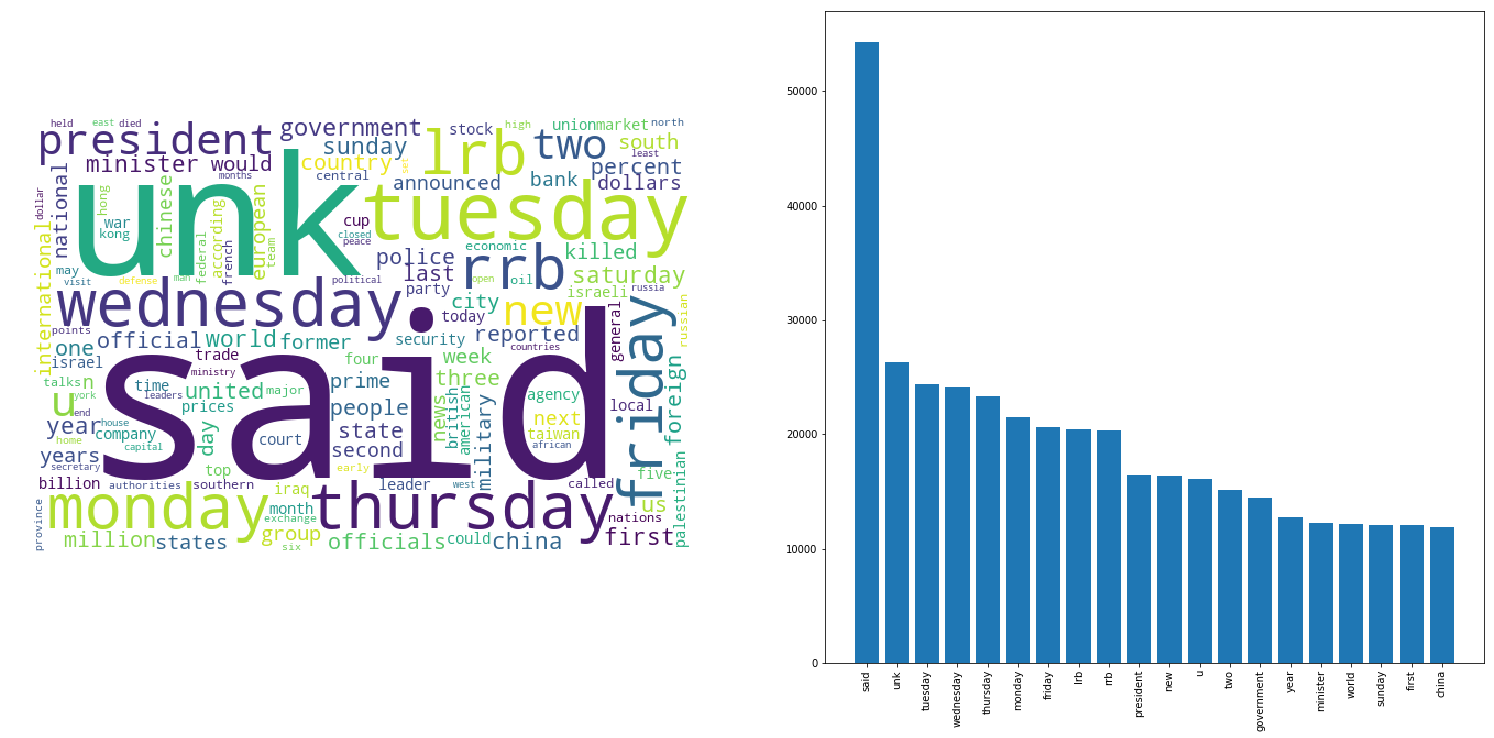
\includegraphics[width=0.7\columnwidth]{sr-eda-gigaword-valid-words}
\centering
\caption{Training and Validation words in the Gigaword dataset}
\end{figure}

In contrast to WikiText, there are a smaller number of domain-specific
words and instead more words similar to those typically used in news
articles, "said", "government", "stock", "tuesday", etc.

\begin{figure}[!ht]
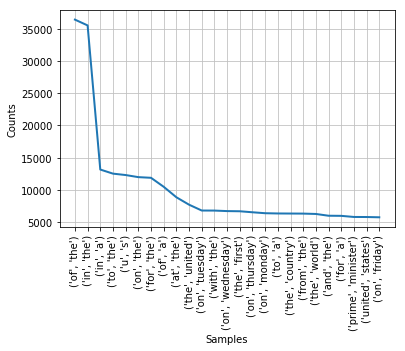
\includegraphics[width=0.7\columnwidth]{sr-eda-gigaword-bigrams}
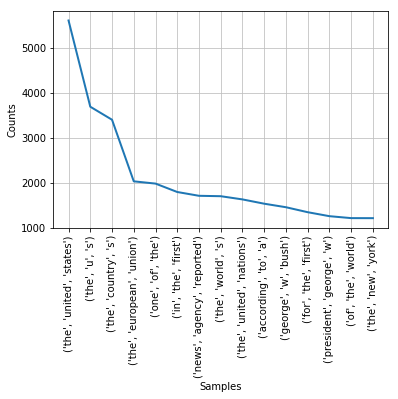
\includegraphics[width=0.7\columnwidth]{sr-eda-gigaword-trigrams}
\centering
\caption{Bigrams and Trigrams words in the Gigaword training set}
\end{figure}

Also notice that bigrams and trigrams for this dataset reveal that a
large number of articles are talking about the same thing, for instance
"the united states", "the european union" and "george w bush".

\section{Metrics}
\label{sec:metrics}

Models are evaluated by taking a sequence
of words from the validation set, removing
$k$ words from the end of the sentence and predicting
the next $k$ words from the existing $n - k$ word sequence.

\subsection{Perplexity}
\label{sec:perplexity}

Perplexity is a measure of "how generalized" the language
model is. A higher perplexity indicates a greater uncertainty
was encountered when predicting sequences of words. Formally,
it is the inverse probability of a text sequence normalized
by the number of tokens.

$$ PP(W) = \sqrt{\prod \frac{1}{P(w|w_1, ..., w_{i - 1}}} $$

Note that perplexity is an "intrinsic metric", it does not
have anything to do with the quality of the predicted
sentences, but instead is based on the certainty of the
model itself.

\subsection{ROUGE}
\label{sec:rouge}

In contrast, metrics such as ROUGE (which is an improvement
on BLEU) measure the quality of a sentence in terms of
their similarity to human generated language. These metrics
are called "extrinsic metrics".

The most basic form of such extrinsic metric is "word error
rate" (WER), defined as:

$$ WER = \frac{S + D + I}{N} $$, where $N$ is the number of
words and $S, D, I$ are substitutions, deletions, insertions.

However, such a metric doesn't take int account the fact that
a recognized sequence may differ in length to a reference
sequence.

Improving on this situation, ROUGE measures based on the
longest matching subsequences, overlapping pairs and n-gram
co-occurrences.

\subsection{METEOR}
\label{sec:meteor}
Another metric trying to improve BLEU is
METEOR. The novel thing about this metric is the use of Recall as well as
Precision to compute the score. It computes the harmonic mean of Recall and
Precision over uni-grams, the weight for recall being higher than Precision,
meaning that false negatives (having a low probability for the true word trying
to predict) will have a big impact on the metric (the score will be lower as the
amount of false negatives increase).

More formally, Precision over an uni-gram is computed as: $$P={\frac
{m}{w_{{t}}}}$$ Where m is the number of uni-grams in the candidate translation
that are also found in the reference translation, and $w_t$ is the number of
uni-grams in the candidate translation.

Recall is computed as: $$R={\frac {m}{w_{{r}}}}$$ Where m is as above, and
$w_{{r}}$ is the number of uni-grams in the reference translation. Precision and
recall are combined using the harmonic mean in the following fashion, with
recall weighted 9 times more than precision: $$F_{{mean}}={\frac {10PR}{R+9P}}$$


\subsection{Naive Accuracy}
Accuracy is measured naively by comparing
a validation set sentence to a predicted sentence and
seeing how many words the model predicted correctly.

\section{Models}
\label{sec:models}

\subsection{RNN}
\label{sec:lstm}

A simple RNN (Elman network) as described in the Milkolov
paper consists of a single linear layer and non-linear
activation (in our case, the $tanh$ function, $ \frac{e^{2x} - 1}{e^{2x} + 1} $, with domain $[ -\infty, \infty ]$ and
range $ [-1, 1] $. The inputs to the network are
a hidden state vector, $h_{t}$, where the size is a hyperparameter
and the input encoding vector $i_{t}$. The output of the network
is the updated hidden state vector $h_{t + 1}$, which will will
be passed as the hidden state vector when processing the $i_{t + 1}$th
word, and the output encoding vector $o_{t}$, which can be
viewed as a discrete probability distribution for the predicted word
at $t$ by applying the softmax function $ \frac{e^x}{\sum e^x_i} $.

The trainable parameters of the RNN are the weights of the linear
layer which determine how information from the previous state of the
hidden state vector and the incoming word vector encoding are encoded
into both the updated hidden state vector and output word vector encoding.

The RNN is trained via "back-propagation through time" (BPTT), which is
effectively the same as the back-propagation algorithm proposed for feed-forward
neural networks, but applied to the recurrent structure of the RNN. In effect,
BPTT involves the same application of the chain rule to recurrent function
applications, and hidden layer states, but usually with some sort of threshold
to prevent computational complexity scaling with the number of tokens the
network has seen so far. In practice this means that the hidden layer encodes
a context window \emph{up to} to a certain length, but no longer than
that length.

Unfortunately, Elman Network RNNs are not able to retain all the optimal
contextual in practice. The reasons for this are given by \cite{Bengio94},
but in summary the issue is that as we backpropagate through time the gradients
from states "further back" in the history start to get vanishingly small, meaning
that they can be easily disrupted by noise or newer information. This means
that the hidden layer doesn't retain long-term information since it is easily
disrupted by new information.

\subsection{LSTM}
\label{sec:lstm}
In contrast to Elman RNNs, LSTM cells remember long-term information "by default" \cite{hochreiter97}.
The hidden state isn't regenerated from the old hidden state and new information coming
through the input, but rather is updated by deleting information and adding new
information.

The LSTM cell uses four "gates" to manage the state of the memory. Each of these
gates comprises a set of weights and activations, descibed below \cite{colah2015}.

The LSTM cell builds upon the basic RNN cell
and adds some gates in order to control how information is stored or deleted.
These gates are element-wise operations, meaning that every value of the hidden
state have a dedicated gate deciding the fate of that value in the next time
step. All the gates are computed taking on account the last hidden state and the
new input and they are applied onto the last hidden state.

The first gate applied is a "forget" gate that regulates how much of the last
hidden state is conserved in this time step. Say that the hidden state contained some
sort of representation as to a place or a point in time, but a new place or point in time arrived.
The forget gate would, in theory, be optimized to notice the new place or point in time and delete
the old place or point in time, otherwise leaving the contextual information unchanged. The output
of the forget gate is activated by the sigmoid function which creates a mask of what information
to retain from the hidden state ($f_t$).

The second one is an "input" gate that decides how much of the new input is encoded into the hidden state.
The activations for the gate by sigmoid essentially form a "mask" which the new input feature vector
$C_t$ gets multiplied by (in order to select the relevant features) ($i_t$).

In order to update the hidden state, we multiply the old hidden state ($h_{t - 1}$) by $f_t$
(masking out the information we want to forget) and multiply the input state by $i_t$, masking in
the information we want to keep, and add them together.

The last gate is an "output" gate which decides which parts of the hidden state are
taken on account to compute the output. The hidden state is first activated by sigmoid to determin
the mask ($o_t$), then the hidden layer is activated by tanh to push the values between $[-1, 1]$, then
finally multipled by the mask $o_t$ in order to determine the output of the network.

The end result with such a variation is that the hidden state is "protected" from perturbation
by virtue of being combined through a single linear layer and activation layer with the input
state on every timestep. Instead, the hidden state is more "explicitly" modified when the
optimized input and forget gates explicitly indicate that information should be added or removed
to the state \cite{hochreiter97}.

The output from the output gate passes through a softmax layer to get the prediction for that time step.

Thanks to this procedure, hidden units can be ignored by the output gate and
they can propagate forward in time without being multiplied by a weight matrix
and applied an activation function at every time step, helping overcome the
gradient vanishing problem.

The forgetting and storing gates help encoding only relevant information into
the hidden state, improving long-time dependencies recall.

Note that the hidden state accuracy benefits here come with a computational compleixty cost - every
LSTM cell has three internal linear layers and five activations, which we pay for both in the forward
pass and in backpropagation through time.

\subsection{GRU}
\label{sec:gru}

In contrast with the LSTM model, Gated Recurrent Unit (GRU) \cite{cho2014} is a simplified
LSTM cell in which the forget and store gates are combined into one "update" gate with complementary
gated values (they sum up to 1 for every hidden unit). This means that the hidden state will
"forget" some information only if it is going to learn some new information. The GRU also
introduces a "reset gate". The "reset gate" is computed by taking the sigmoid of the sum of weighted
inputs and hidden state
 $\sigma ([ W_r d x]_j + [ U_r  h - 1])$.

When the "reset gate" is close to zero, the entire hidden state is thrown away and reset with
the current input gate state.

The net effect is that the GRU can learn short term dependencies between inputs
over different timescales. The units that capture short term dependencies frequently
activate the reset gate, whereas the units that learn long term dependencies have
more active update gates \cite{cho2014}.

\section{Encoding and Decoding}
\label{sec:encdec}

\subsection{Embeddings}
\label{sec:embedddings}

Traditionally, the Language Models were feeded each word as a One-Hot encoded vector as large as the
vocabulary is. Since vocabularies can be really large (20k to 800k for languages
with many compounded words such as Finnish), this presents a computational
problem, large matrices multiplication is expensive. Word Embeddings provide an
alternative procedure in which the words to be fed to the network are encoded
in an $n$ dimensional space. The embedding layer can learn a word encoding such
that words related to each other semanticaly, get similar encoded vectors after
the transformation. Even some basic arithmetic is possible by adding and subtracting the euclidean distance of vectors. For example, if you
subtract (the vector for "queen" - the vector from "woman") from the vector for "king" you get the vector
for "man".

Word embeddings can be learned end-to-end with a single training
process, as long as there is some task giving the words a representation in a domain,
for instance, predicting the next word, which a language model is designed to do. This
means that the word embeddings need not be trained separately but can be learned
as part of the process of training the entire language model as a separate layer.

Word embeddings also have the distinct advantage that they can reduce both training
and inference complexity because fewer multiplications need to be done at
the RNN, LSTM or GRU cell phase both at the inference and training time. The
comptutation of the embedding layer can be heavily optimized because the relevant
input will only have a non-zero value in a single vector component.

\begin{figure}[!ht]
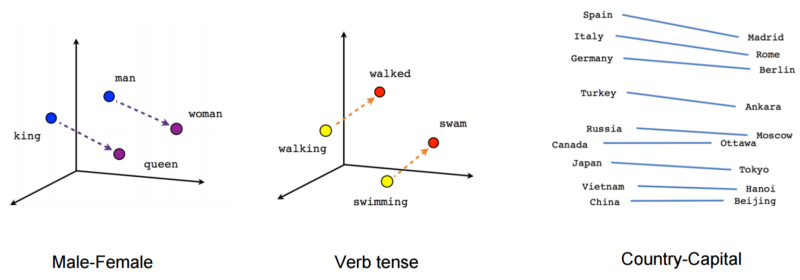
\includegraphics[width=\textwidth]{01}
\centering
\caption{Three embedding vector spaces showing how euclidean distance is following the semantic relations for: a) male and female. b) verb tenses. c) countries and capitals }
\end{figure}

\subsection{Shortlists}
\label{sec:shortlists}

Like embeddings, shortlists also provide a way to reduce the computational
complexity, but this time at the output layer instead of the inference layer
\cite{schwenk05}. In the shortlist we pick the $n$ most frequent words in the
corpus and $n$ output units to those $n$ words in the corpus, predicting every
other uncommon word as an unknown token. However, input encodings still
allow for representations of those words deemed uncommon, either by
embeddings or one-hot encoding.

The overall theory behind shortlists is that any optimal model operates
on a pareto principle, 20% of the words which are the most frequent will
be predicted roughly 80% of the time. Since the computation of the output
encodings of height $|V|$ is a fixed cost on every training and inference
cycle, the user of the model is paying for the capacity to predict words which
will seldomly be predicted. A good shortlist should be able to substantially
reduce the computational complexity of the model whilst still retaining a
relatively high degree of accuracy.

\section{Regularization}
\label{sec:regularization}

The Milkolov paper flags that performance on the validation could not be
improved by using "standard regularization procedures" (we assume that
the paper must have been referring to L1 or L2 regualrization based on the
techniques in existence at the time) \cite{Milkolov10}. We propose that a
popular regularization technique known as "Dropout" may be of some assitance.

\subsection{Dropout}
\label{sec:dropout}

Dropout \cite{hinton2012} is the probabilistic approximation of an ensemble
of the power-set of weights in a Neural Network. In the words of Hinton, it
reduces overfitting by reducing "complex co-adaptations on the training data",
meaning that the network does not depend too much on the activation of
certain sets of units in order to produce the majority of activations, instead
ensuring that every unit is utilized roughly equally. In the case of language models,
this should in principle prevent the network from just recalling the training data.

\subsection{Tied Weights}
\label{sec:tiedweights}

Another regularization technique addresses the parameters in the encoder and the decoder. In our models, both of these layers have the vocabulary size as one of their dimensions. The encoder transforms the (vocabulary sized) one-hot encoding into a word encoding while the decoder transforms the hidden state into a softmax as big as the vocabulary size. These sizes can get huge as the vocabulary can contain from 20k to 800k with languages with many compound words (such as Finnish), which means that overfitting is quite likely as many of the parameters included in encoder and decoder may be redundant.

In order to help solving this issue, Press O. et al \cite{press16} proposed sharing the same weights for encoder and decoder, as one is the same size as the transpose of the other and both perform a translation between a dense encoded layer and a sparse one. They showed in their work how this technique can reduce the number of parameters in the model without hurting the performance while lowering the perplexity score.

\section{Initialization}
\label{sec:initialization}

The starting values for the model parameters play a significant role in the training process for RNNs. The reason is mainly due to the depth these models reach while propagating through time. As the hidden state travels from time step to the next, an activation function is applied. The compound effect of performing the activation function several times tend to take the hidden state value towards the saturation zone of the activation functions. In order to avoid the saturation of the hidden units, the starting values must be chose carefully to ensure a correct behavior from the beginning, starting the training with as many active units as possible.

\subsection{Xavier}
\label{sec:xavier}

Xavier initialization \cite{xavier10} was designed for the sigmoid and tanh functions. This is the initialization relevant to us since we have applied such functions more than the RELU.
Xavier initialization consists on starting the hidden state values as a random distribution with variance as follows:
$$var = \sqrt{\frac{1}{size_h}}$$

Where $size_h$ is the number of hidden units. This ensures that the variance at the next hidden state is the same as the variance at the previous one. Maximizing the probability of having hidden units close to the mean and therefore out of the saturation zones.

\section{Model Configurations and Results}
\label{sec:results}

We ran two sets of experiments on each dataset. Because of the difference in sizes
between the Gigaword and WikiText datasets we were able to run more tests on the
WikiText dataset and scale a few of those results up to Gigaword.

\subsection{Performance by Model Architecture}
\label{sec:perf_by_model_arch}

\begin{figure}[!ht]
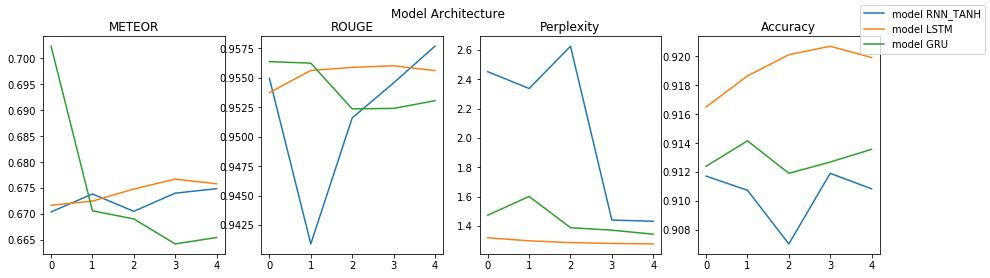
\includegraphics[width=0.7\columnwidth]{sr-perf-by-model-architecture}
\centering
\caption{Validation Set Performance by Model Architecture on WikiText}
\end{figure}

Comparing each of the three models with 200 hidden units, 2 layers and
no dropout or embeddings, trained to five epochs in batches of 200 sentences at a
time, we see that the LSTM model generally outperforms all three on all metrics.
It has the lowest overall perplexity, highest METEOR score after five iterations
and highest overall naive accuracy, scoring roughly one half a percentage point
higher than the other two models.

\subsection{Performance by number of hidden layers}
\label{sec:perf_by_n_layers}

\begin{figure}[!ht]
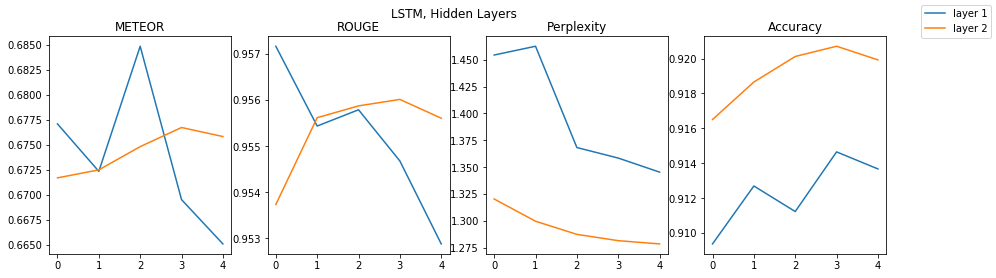
\includegraphics[width=0.7\columnwidth]{sr-perf-by-hidden-lstm}
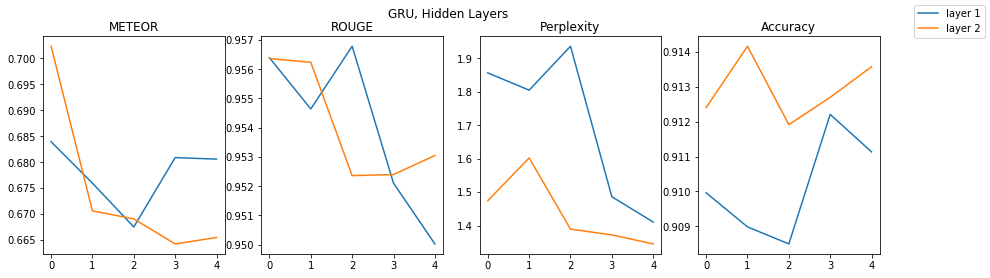
\includegraphics[width=0.7\columnwidth]{sr-perf-by-hidden-gru}
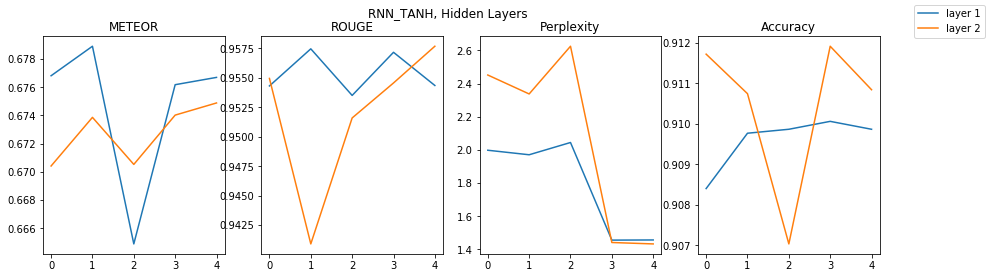
\includegraphics[width=0.7\columnwidth]{sr-perf-by-hidden-rnn}
\centering
\caption{Validation Set Performance by number of Hidden Layers on WikiText}
\end{figure}

We measured differences in performance with both one and two hidden layers
on the RNN cell for each model architecture with 200 hidden units per cell, trained
to five epochs in batches of 200 sentences at a time.

In general, we find that increasing the number of hidden layers on the network
increases performance on all metrics, probably because the model is able to
encode more information from the training set in its layers recurrent layers.

We notice that in the Elman Network RNN training was generally unstable and
increasing the number of layers gave inconclusive results.

\subsection{Performance by number of hidden units}
\label{sec:perf_by_n_hidden}

\begin{figure}[!ht]
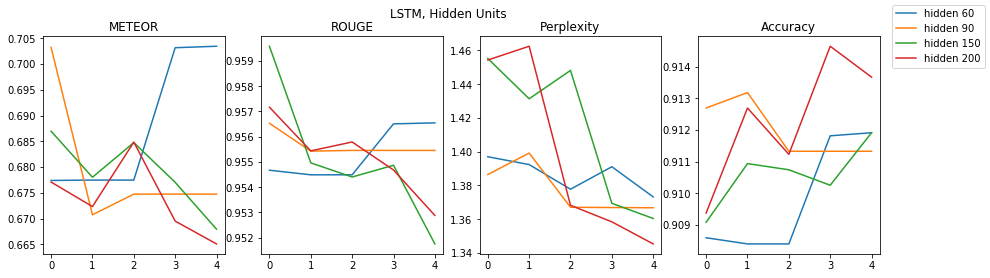
\includegraphics[width=0.7\columnwidth]{sr-perf-by-hidden-units-lstm}
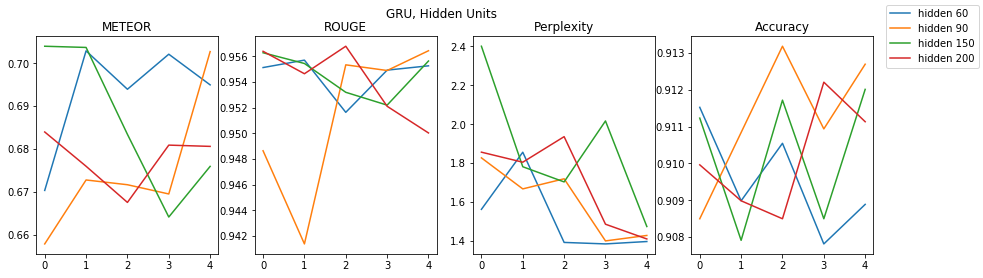
\includegraphics[width=0.7\columnwidth]{sr-perf-by-hidden-units-gru}
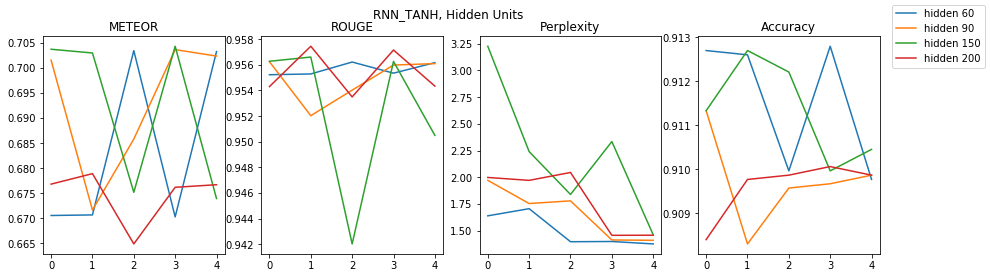
\includegraphics[width=0.7\columnwidth]{sr-perf-by-hidden-units-rnn}
\centering
\caption{Validation Set Performance by number of Hidden Units on WikiText}
\end{figure}

We measured differences in performance with 60, 90, 150 and 200 hidden units per
RNN cell for each model architecture with 1 RNN cell, trained
to five epochs in batches of 200 sentences at a time.

In general we found that like increasing the number of layers,
increasing the number of hidden units per layer can help with overall accuracy,
but not as much as increasing the number of layers does. In fact, having a fewer
number of hidden units may act as a regularizer which would help to prevent
overfitting and improve accuracy on the validation data.

\subsection{Performance by Dropout}
\label{sec:perf_by_dropout}

\begin{figure}[!ht]
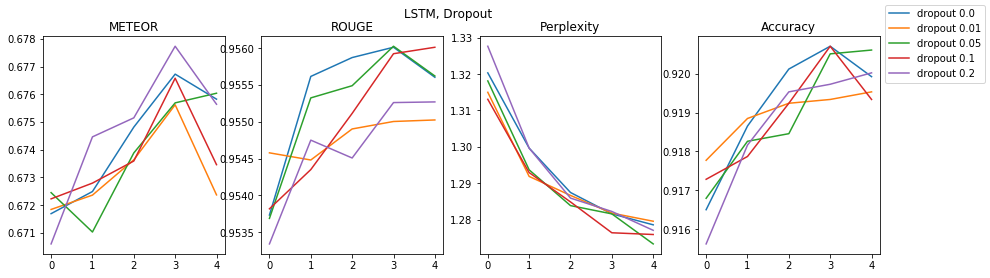
\includegraphics[width=0.7\columnwidth]{sr-perf-by-dropout-lstm}
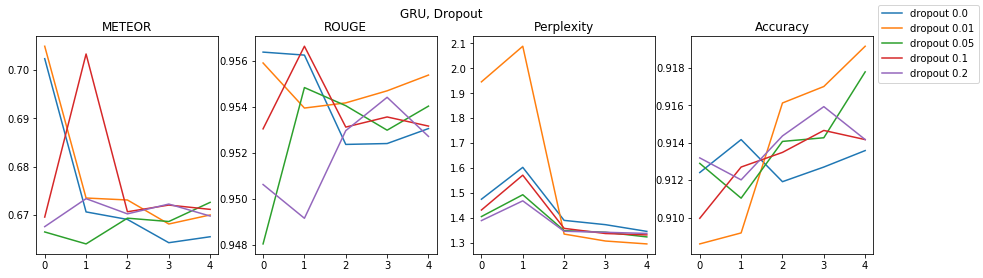
\includegraphics[width=0.7\columnwidth]{sr-perf-by-dropout-gru}
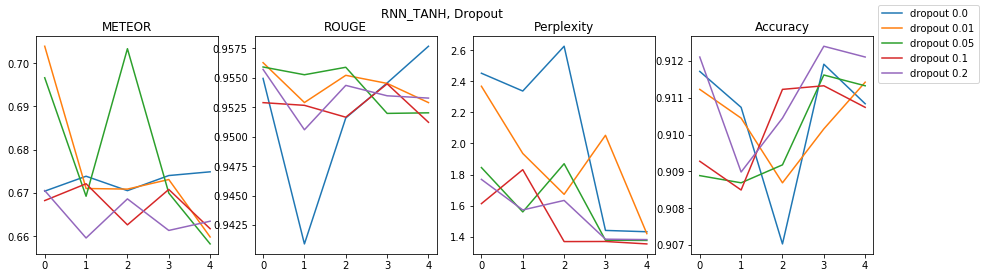
\includegraphics[width=0.7\columnwidth]{sr-perf-by-dropout-rnn}
\centering
\caption{Validation Set Performance by Dropout Probability on WikiText}
\end{figure}

We measured differences in performance with dropout probabilities
0.0, 0.01, 0.05, 0.1, 0.2 per RNN cell for each model architecture with
1 RNN cell, 200 hidden units, trained to five epochs in batches of 200
sentences at a time.

For GRU cells, we find that small amounts of dropout (0.01-0.05) can act
as an effective regularizer and improve accuracy and ROUGE scores on unseen
data by a few tenths of a percentage point. For LSTM cells we find that
dropout did not assist all that much, indicating that perhaps those models were
not already starting to overfit by five epochs. For RNN cells, we observed
that again, training was quite unstable that it was difficult to observe what
difference, if any, dropout had on the metrics.

\subsection{Performance by Embedding Dimensions}
\label{sec:perf_by_embedding}

\begin{figure}[!ht]
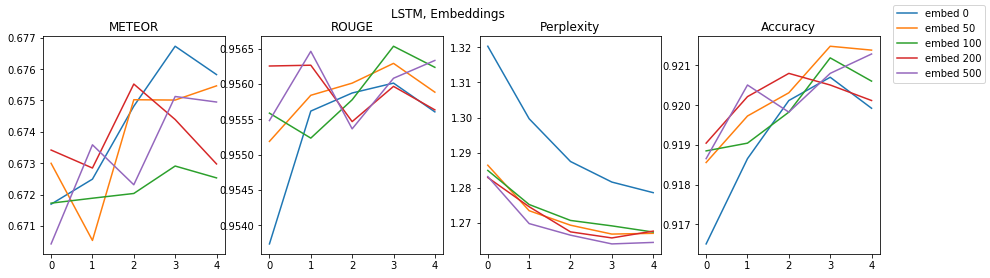
\includegraphics[width=0.7\columnwidth]{sr-perf-by-embedding-lstm}
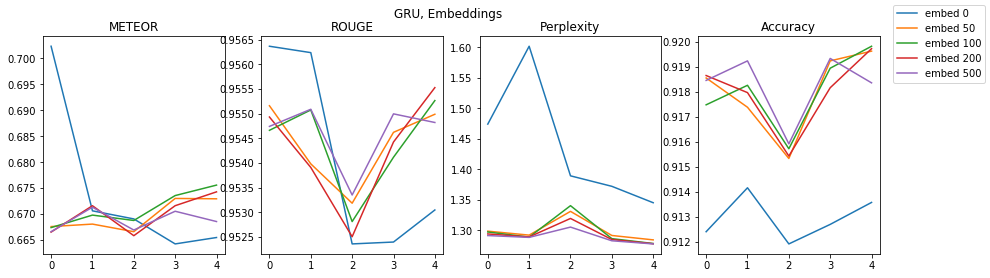
\includegraphics[width=0.7\columnwidth]{sr-perf-by-embedding-gru}
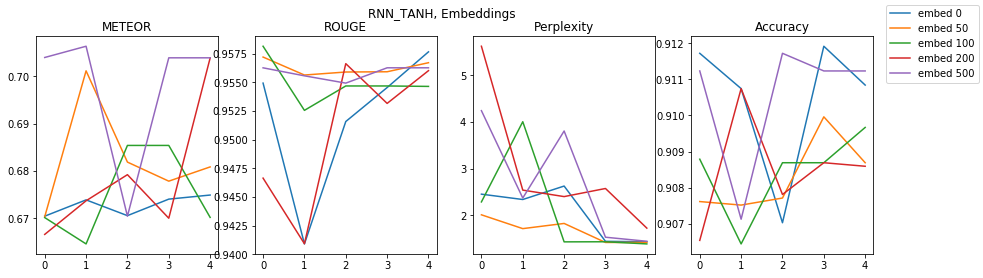
\includegraphics[width=0.7\columnwidth]{sr-perf-by-embedding-rnn}
\centering
\caption{Validation Set Performance by Embedding Dimension on WikiText}
\end{figure}

We measured differences in performance with embedding sizes 0, 50,
100, 200 and 500 at the encoder layer for each model architecture with
1 RNN cell, 200 hidden units, trained to five epochs in batches of 200
sentences at a time.

On both LSTM and GRU models, any use of encoder embeddings noticably outperformed
one-hot encoding on almost all metrics, except METEOR for LSTMs. It seems to be
the case that the learned embeddings encoded useful information about the
non-temporally dependent relationships between words. For Elman RNN cells, we
again observed that because training was so unstable, embeddings did not
appear to make much of a difference to accuracy, even if they result in
much lower computational complexity.

\subsection{Performance by Shortlist Dimension}
\label{sec:perf_by_shortlist}

\begin{figure}[!ht]
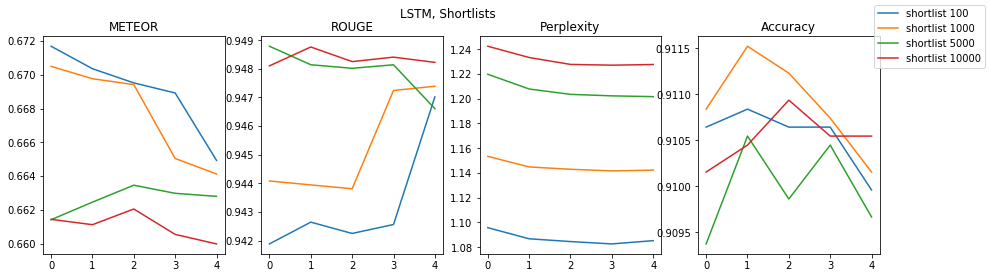
\includegraphics[width=0.7\columnwidth]{sr-perf-by-shortlist-lstm}
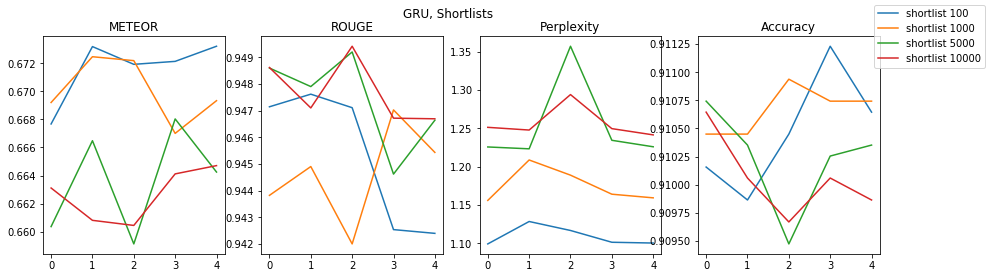
\includegraphics[width=0.7\columnwidth]{sr-perf-by-shortlist-gru}
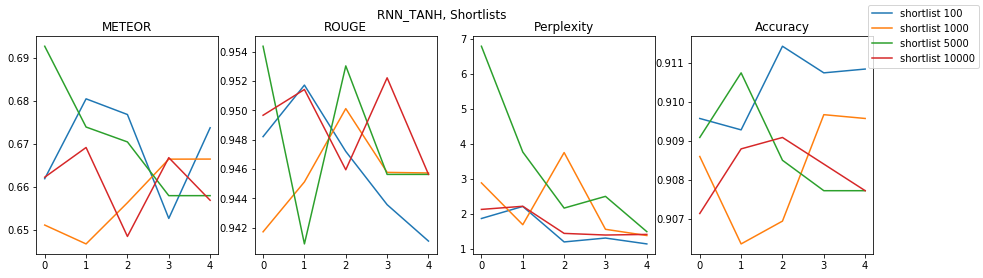
\includegraphics[width=0.7\columnwidth]{sr-perf-by-shortlist-rnn}
\centering
\caption{Validation Set Performance by Shortlist Dimension on WikiText}
\end{figure}

We measured differences in performance with shortlist sizes 100, 1000, 5000, 1000
at the decoder layer for each model architecture with 1 RNN cell, 200 hidden units and
an input encoder embedding size of 500, trained to five epochs in batches of 200 sentences at a time.

On WikiText, note that the original corpus contained 28,755 words in its
dictionary and achieved accuracy scores of 0.921 for the LSTM, 0.918 for the GRU
and 0.911 for Elman RNN.

By contrast, shortlists for LSTM, GRU and Elman RNNs
achieve accuracy scores between 0.910 and to 0.911,
with larger shortlists marginally outperforming smaller
shortlists. This indicates that a large proportion of
the words being predicted on the non-shortlisted
models are likely to be very frequent words, meaning
that if we \emph{only} allow the network to predict
frequent words by shortlisting then we can still get
slightly worse but similar performance.

\subsection{Performance by Tied Weights}
\label{sec:perf_by_tiedweights}

We measured performance with tied weights, word embedding of size 200 and 2 hidden layers of size equal to the word embedding (200), this is a requirement for the encoder and decoder must have the same size in order to tie their weights. We trained to five epochs in batches of 200 sentences at a time.
 
For the implementation of Tied Weights we were expecting lower perplexity levels as well as a small improvement or no change on the other metrics, however the LSTM and GRU models didn't show any perplexity improvements while the other metrics got worse. Our implementation of tied weights had a negative impact. For the tanh model as small perplexity improvement is shown but the other metrics are very unstable to draw any conclusions from them.

\begin{figure}[!ht]
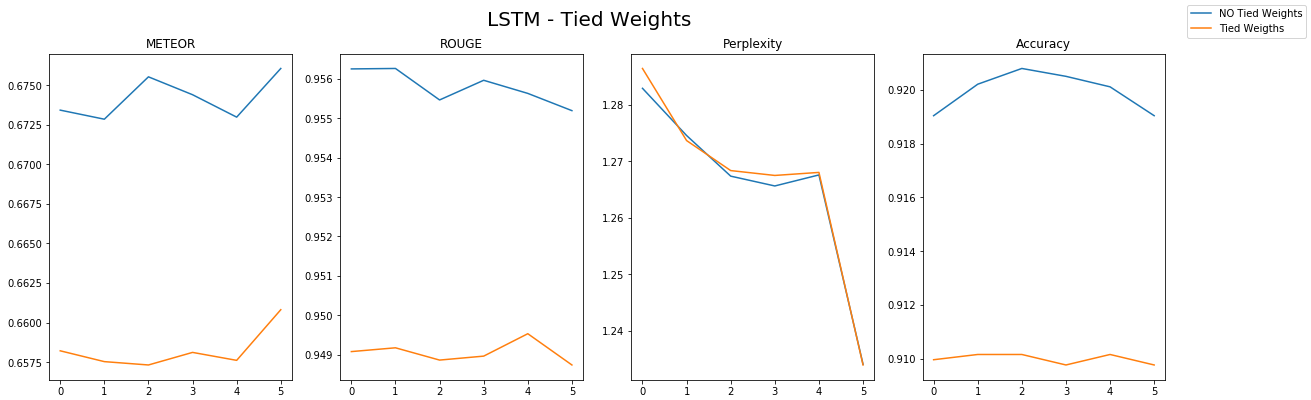
\includegraphics[width=\textwidth, height=3cm]{lstm-tw}
\centering
\end{figure}
\begin{figure}[!ht]
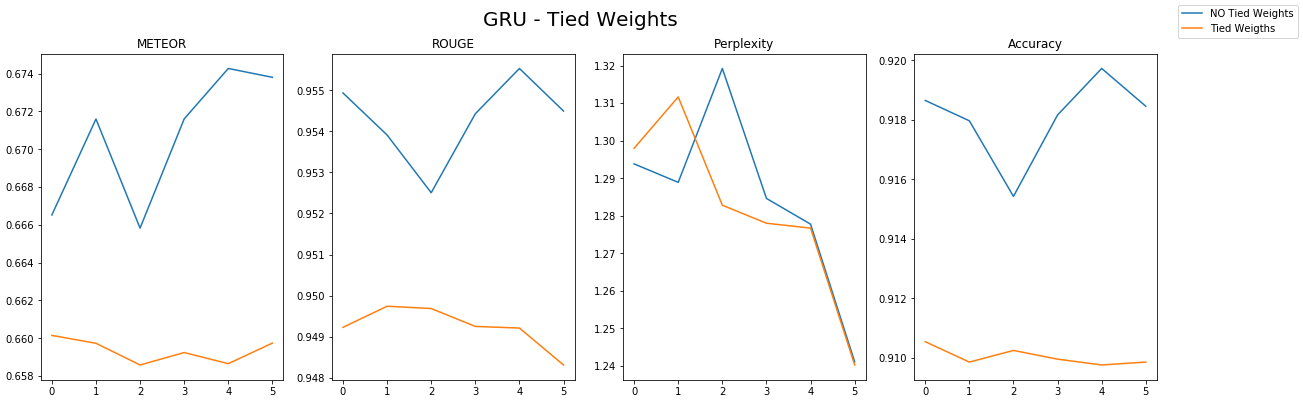
\includegraphics[width=\textwidth, height=3cm]{gru-tw}
\centering
\end{figure}
\begin{figure}[!ht]
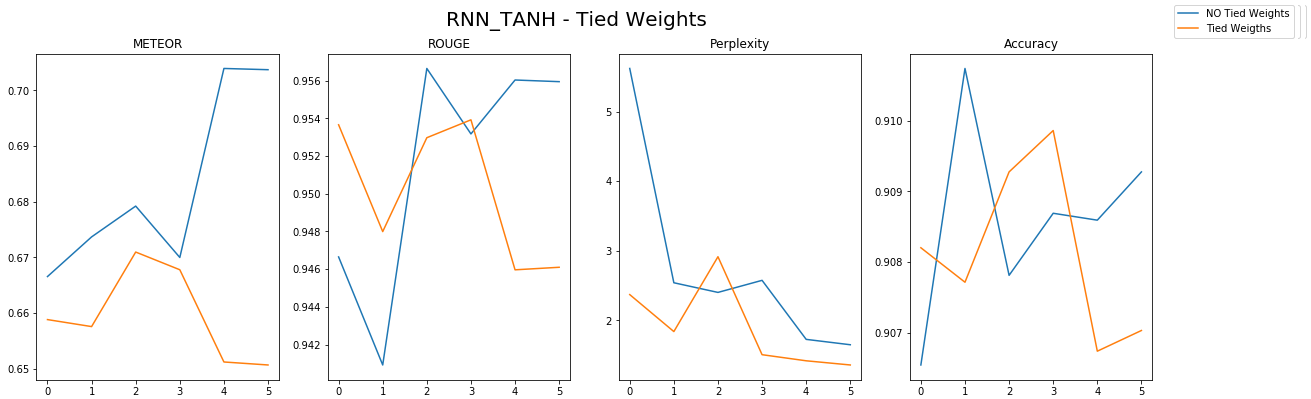
\includegraphics[width=\textwidth, height=3cm]{tanh-tw}
\centering
\caption{Validation Set Performance by Model on WikiText for Tied Weights}
\end{figure}


\subsection{Performance by Xavier Initialization}
\label{sec:perf_by_xavier_init}

We measured performance with Xavier initialization, word embedding of size 500 and 2 hidden layers of size 200.
We trained to five epochs in batches of 200 sentences at a time.
 
In all three models we get worse results when implementing Xavier initialization. The perplexity is not modified
by much but METEOR, ROUGE and Naive Accuracy are clearly worse. Analysis of the activation function values across training steps
would be needed to determine why Xavier initialization wasn't able to improve the results.

\begin{figure}[!ht]
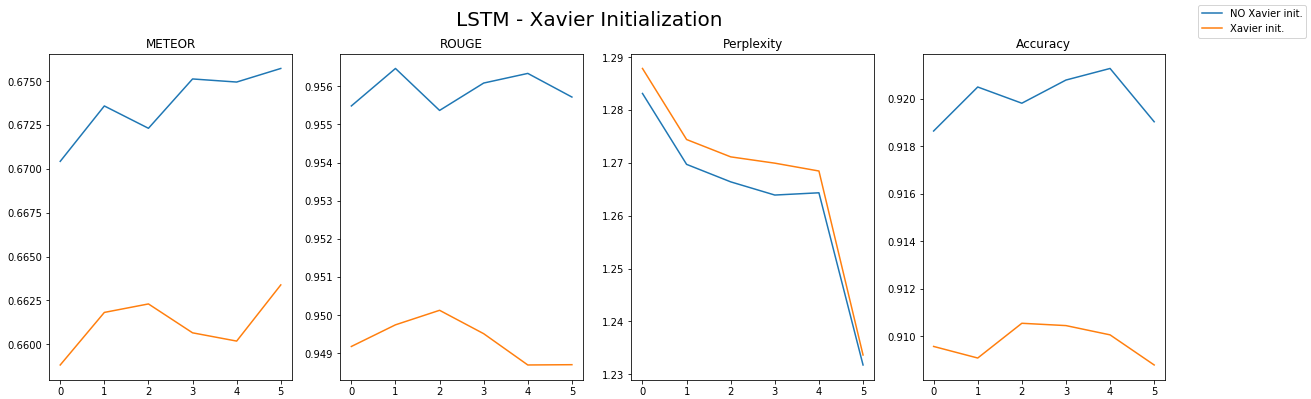
\includegraphics[width=\textwidth, height=3cm]{lstm-xi}
\centering
\end{figure}
\begin{figure}[!ht]
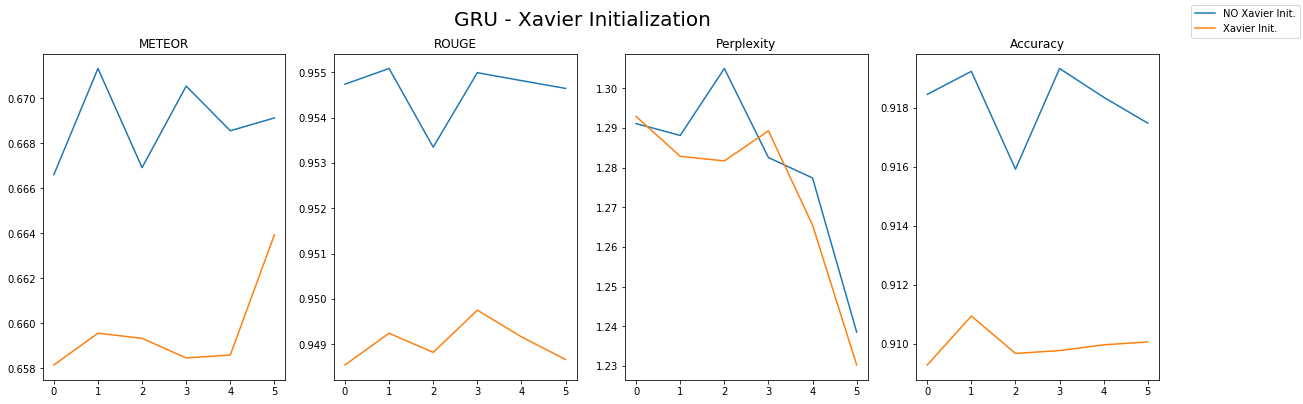
\includegraphics[width=\textwidth, height=3cm]{gru-xi}
\centering
\end{figure}
\begin{figure}[!ht]
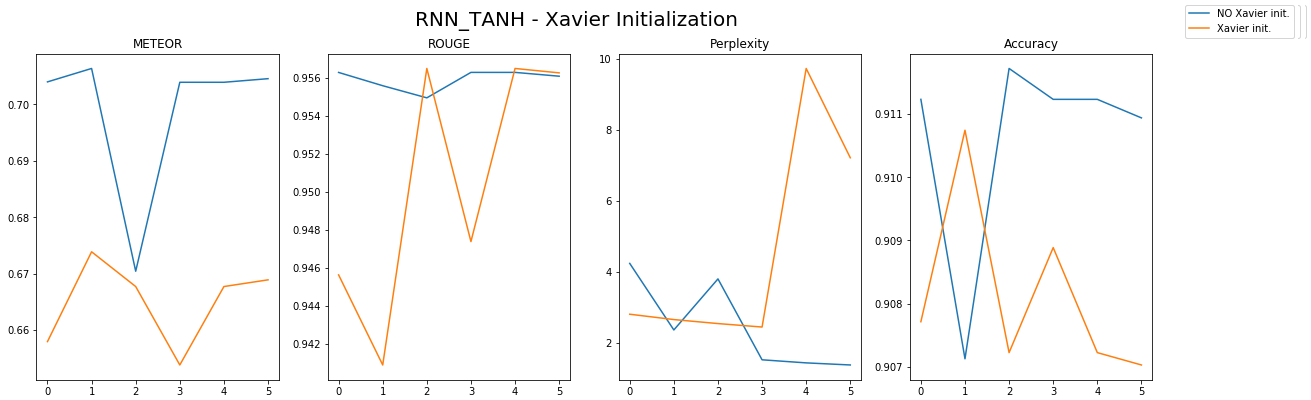
\includegraphics[width=\textwidth, height=3cm]{tanh-xi}
\centering
\caption{Validation Set Performance by Model on WikiText for Xavier Initialization}
\end{figure}


\section{Analysis}
\label{sec:analysis}

\section{Future Work}
\label{sec:future}

\begin{thebibliography}{9}
\bibitem{nano3}
  K. Grove-Rasmussen og Jesper Nygård,
  \emph{Kvantefænomener i Nanosystemer}.
  Niels Bohr Institute \& Nano-Science Center, Københavns Universitet


\bibitem{Bengio94}
  http://ai.dinfo.unifi.it/paolo//ps/tnn-94-gradient.pdf

\bibitem{hochreiter97}
  http://www.bioinf.jku.at/publications/older/2604.pdf

\bibitem{schwenk05}
  ftp://tlp.limsi.fr/public/emnlp05.pdf. Accessed 6 Nov. 2018.
  
\bibitem{Milkolov10}
  Milkolov T., et al, Recurrent neural network based language model, INTERSPEECH 2010
  
\bibitem{xavier10}
  Understanding the difficulty of training deep feedforward neural networks - Glorot, Xavier \& Bengio Yoshua. 2010

\bibitem{hinton2012}
  https://arxiv.org/pdf/1207.0580.pdf

\bibitem{cho2014}
  https://arxiv.org/pdf/1406.1078v3.pdf
  
\bibitem{colah2015}
  http://colah.github.io/posts/2015-08-Understanding-LSTMs/

\bibitem{press16}
  Using the Output Embedding to Improve Language Models - Press, Ofir \& Wolf, Lior. 2016

\end{thebibliography}


\end{document}
